\documentclass[tikz,border=2mm]{standalone}
\usepackage{tikz}
\usepackage{pgfplots}
\pgfplotsset{compat=1.18}

\begin{document}
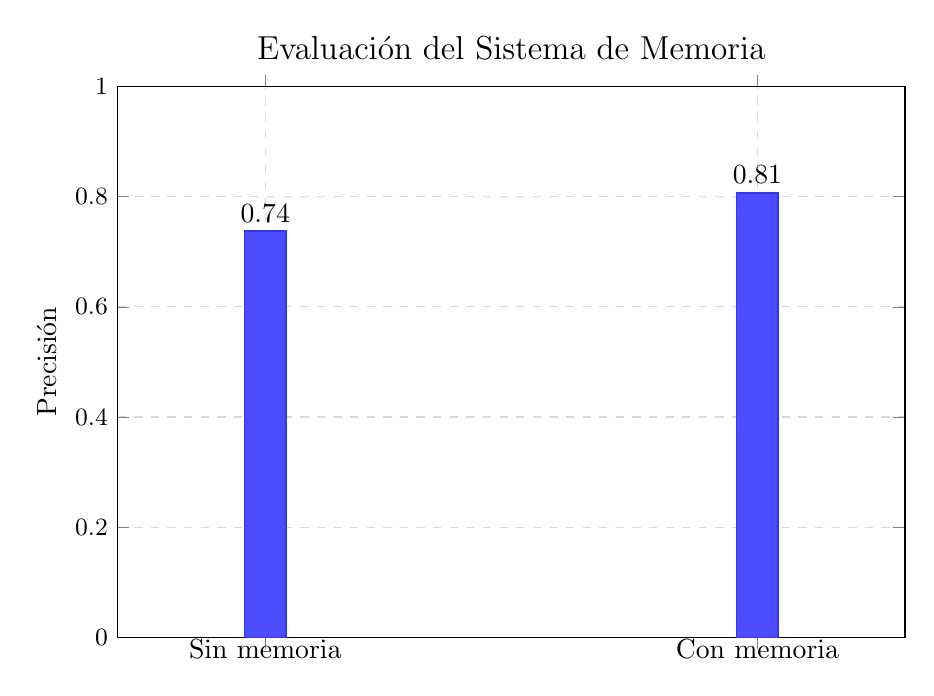
\begin{tikzpicture}
\begin{axis}[
    title={Evaluación del Sistema de Memoria},
    title style={font=\large},
    ylabel={Precisión},  
    xlabel=,
    ymin=0,
    ymax=1.0,
    ytick={0,0.2,0.4,0.6,0.8,1.0},
    enlarge x limits=0.3,
    ybar=4pt,
    bar width=15pt,
    symbolic x coords={Sin memoria, Con memoria},
    xtick={Sin memoria, Con memoria},
    x tick label style={rotate=0, anchor=center, font=\normalsize},
    yticklabel style={font=\small},
    width=10cm,
    height=7cm,
    grid=major,
    grid style={dashed, gray!30},
    tick label style={font=\normalsize},
    scale only axis,
    ylabel style={font=\normalsize},
]
\addplot[
    fill=blue!70,
    draw=blue!80,
    line width=0.5pt
] coordinates {
    (Sin memoria, 0.7377)
    (Con memoria, 0.8066)
};

% Añadir valores sobre las barras
\node at (axis cs:Sin memoria,0.77) {\normalsize 0.74};
\node at (axis cs:Con memoria,0.84) {\normalsize 0.81};



\end{axis}
\end{tikzpicture}
\end{document}
